\documentclass{article}
\usepackage[utf8]{inputenc}
\usepackage[inner=3cm,outer=3cm,top=3.0cm,bottom=3.0cm]{geometry}
\usepackage[british,UKenglish,USenglish]{babel}
\usepackage{graphicx}
\usepackage{subcaption}
\usepackage{amsmath}
\usepackage{amssymb}
\usepackage[backend=biber,style=numeric,sorting=none]{biblatex}
\addbibresource{references.bib}

\DeclareMathOperator*{\argmin}{\arg\!\min}
\newcommand{\norm}[1]{\left\lVert#1\right\rVert}
\usepackage{graphicx}

\title{Machine Learning - Miniproject 2 \\ \Large Classification of the Digits Dataset}
\author{Diogo Cosin and Ralph Florent}
\date{April 21, 2019}

\begin{document}

\maketitle

% \begin{abstract}
% In this project, we classify the Digits data set through a full data processing pipeline. Firstly, K-means is used to reduced the raw data dimensionality. After the feature extraction stage, a Ridge regression classifier is trained. Its performance is assessed through the metrics Misclassification and Mean Standard Error. The classifier performance is also optimized by tuning the number of K-means clusters and the ridge factor $\alpha^2$ through a grid search strategy. Finally, after the best model is defined according to its performance metrics, the model is validated using a completely new data set.

% \end{abstract}

\section{Introduction}

In this section, we describe the classification task approached in this report. We also briefly discuss some of the theoretical concepts applied during the development and execution of the task.

\subsection{Task Description}

In this project, we classify the Digits dataset through a full data processing pipeline. Firstly, K-means is used to reduce the raw data dimensionality. After this feature extraction stage, a Ridge regression classifier is trained. Its performance is assessed through cross-validation and the metrics Misclassification and Mean Standard Error. The classifier performance is also optimized by tuning the number of K-means clusters and the ridge factor $\alpha^2$ through a grid search strategy. Finally, after the best model is defined according to the performance metrics obtained by the cross-validation, the model is validated using a completely new test data set.

\subsection{Theory Review}

The concepts involved during the task are briefly reviewed in this subsection. Further and more detailed explanations can be verified in the references provided throughout this report.

\subsubsection{Linear Regression Model}

In a linear regression task, one searches for the optimal linear function $d_{opt} \in D$ that minimizes the distance between the predicted and ground truth values, where $D$ is the set of candidate functions. Formally speaking, $d_{opt}$ is obtained according to:

\begin{equation}
    d_{opt} = \argmin_{d_{opt} \in D} \frac{1}{N} \sum_{i=1}^{N} \norm{d(\mathbf{f}_i) - z_i}^2,
\end{equation}

\noindent
where $\mathbf{f}_i$ is the $i_{th}$ feature pattern in the dataset containing $N$ samples and $z_i$, the ground truth for the $i_{th}$ sample \parencite {lecturenotes}.

Therefore a linear function that maps from $m$-dimensional features to $k$-dimensional targets, $d: \mathbb{R}^m \mapsto \mathbb{R}^k$, is a $k \times m$ sized matrix $W$, and the optimal solution $W_{opt}$ respects:

\begin{equation}
    W_{opt} = \argmin_{W_{opt} \in {\mathbb{R}^{k \times m}}} \frac{1}{N} \sum_{i=1}^{N} \norm{W\mathbf{f}_i - z_i}^2 \parencite {lecturenotes}.
\end{equation}

In order to avoid always mapping the zero vector $\mathbf{f}_i = 0$ to the all-zero class indicator, a so-called $bias$ term is added to linear function as:

\begin{equation}
    d(\mathbf{f}_i) = W\mathbf{f}_i + b,
\end{equation}

\noindent
where $b \in \mathbb{R}^{k}$ is the constant $bias$ vector \parencite {lecturenotes}.

A strategy commonly used to generate the $bias$ vector is to, during the feature extraction stage, always map the last feature of the feature vectors $\mathbf{f}_i$ to the constant 1. This way, an offset is inserted into the feature vectors so that the zero vector is not necessarily mapped to the all-zero class indicator \parencite {lecturenotes}.

Returning to the task that seeks the optimal matrix $W_{opt}$, one can show, using Linear Algebra techniques, that $W_{opt}$ can be determined by:

\begin{equation}
    W^{\prime}_{opt} = (\Phi^{\prime}\Phi + \alpha^2 I_{m \times m})^{-1} \Phi^{\prime}Z, \label{eq:w_opt}
\end{equation}

\noindent
where $\Phi$ is obtained arranging the feature vectors row-wisely into a $N \times m$ matrix, while $Z$, arranging the targets into a $N \times k$ matrix. The mathematical derivations of Equation \eqref{eq:w_opt} are beyond the scope of this report \parencite[See][equation 19-26]{lecturenotes}.

\subsubsection{K-means Dimensionality Reduction} \label{sec:k-means}

Besides being an unsupervised learning technique, \textit{K-means} can also be applied as a feature extraction technique. After the \textit{K-means} procedure is executed for \textit{K} clusters, \textit{k codebook} vectors are obtained pointing from the origin to the centroid of each of the $K$ clusters. The feature extraction happens by calculating the Euclidean distance between the data points $x_i$ and the \textit{codebook} vectors $c_i$ and assigning each distance as a new feature. That is, a $n$-dimensional data point $x$ is reduced to a $k$-dimensional feature vector $\mathbf{f}_i$ \parencite {lecturenotes}.

Therefore, given the data points $(x_i)_{i=1,...,N} \in \mathbb{R}^{n}$ and $(c_i)_{i=1,...,K} \in \mathbb{R}^{n}$ codebook vectors of $k$ clusters, applying dimension reduction as mentioned above can mathematically be expressed as follows:

\begin{equation}
	f(x_i, c_i): \mathbb{R}^n \mapsto \mathbb{R}^k, (x_1, x_2,...,x_N) \mapsto (\mathbf{f}_1, \mathbf{f}_2,...,\mathbf{f}_N),
\end{equation}

\noindent
where $\mathbf{f}_i = \norm{x_i - c_j}_{j = 1, 2,..., k}$. Thus, the set of $x_i$ data points are mapped from $n$-dimension to $k$-dimension, $f(x_i) = \mathbf{f}_i$, denoted as feature vectors \parencite {lecturenotes}.

In addition to that, considering that the \textit{bias} factor has also to be inserted into the feature vectors $\mathbf{f}_i$, the K-means feature extraction function $f$ maps a $n$-dimensional vector to a $(k+1)$-dimensional vector \parencite {lecturenotes}. Mathematically speaking, $f: \mathbb{R}^n \mapsto \mathbb{R}^{k+1}$ is defined as:

\begin{equation}
    f(x_{i}) = \mathbf{f}_i, \label{eq:k-means}
\end{equation}

\noindent
for $i=1, 2, ...,N$.

\subsubsection{Principal Component Analysis}
\textit{Principal component analysis (PCA)}, an unsupervised approach, refers to the process by which principal components are computed, and the subsequent use of these components in understanding the data \parencite[see][Section 10.2]{james2013introduction}. In other words, it is a mathematical procedure that transforms a number of possibly correlated variables into a smaller number of uncorrelated variables called principal components \parencite{ncsu}. PCA is considered for this task realization an appropriate method for dimensionality reduction due to its flexibility in interpreting the variance and the correlation between features in this dataset.

\subsubsection{Cross-validation}

Cross-validation is a statistical method used in order to determine the optimal model being trained. The idea behind it is to make use only of the available training data in a way that the model is tested in a completely new data set. In a sense, the cross-validation technique emulates the test data (not touched by the model during the training phase) from the available training data. This way, it is possible to estimate if the model is overfitting or underfitting using only the training data.

How does it work? The technique is simple. The training data is split into two partitions. One partition is then used as the training data, while the remaining one is used as the test data. One may also instead of splitting only into two partitions, splits into \textit{K} partitions, more commonly called \textit{folds}. The model is then trained in the combination of $K - 1$ folds and validated in the remaining \textit{fold}. The procedure is repeated \textit{K} times, which means that each \textit{fold} is used as the test data once. The model is then assessed by taking the average of its \textit{K} performance results. Finally, the optimal model is chosen according to the metrics defined for the machine learning task at hand. This procedure is known as \textit{K-fold cross-validation}. 

However, there is a bias-variance trade-off associated with the choice of $k$ in k-fold cross-validation compared to other cross-validation methods such as \textit{Leave-One-Out Cross-Validation (LOOCV)}. Typically, one performs \textit{k-fold cross-validation} using $k = 5$ or $k = 10$, as these values have been shown empirically to yield test error rate estimates that suffer neither from excessively high bias nor from very high variance \parencite{james2013introduction}.

During the execution of the task presented at this report, the models are chosen using the \textit{K-fold cross-validation} and its performance is evaluated by the metrics Mean Standard Error and Accuracy.

\section{Methodology}

The procedure, as well as the technology utilized during the project, are described in this section. 

\subsection{Data Pipeline}

The project implements a full data processing pipeline. That is, the dataset is extracted from a \textit{.txt} file and converted to a suitable format which can be processed by the next steps of the pipeline. Posteriorly, a feature extraction is performed as described by Equation \eqref{eq:k-means} in Subsection \ref{sec:k-means}. The new feature vectors, obtained after the feature extraction, are then applied to a linear regression classifier and the training, and test results are evaluated through in a \textit{K-fold} cross-validation using 10 \textit{folds}. Finally, the best model, chosen according to the cross-validation results, is retrained in the full training data and evaluated in a new dataset, which is not utilized during the training and cross-validation stages.

To make the pipeline easily understandable, Figure \ref{fig:pipeline} presents a diagram describing the whole process visually. The dimensionality of the data during the process is indicated as the text labels of the arrows.

\begin{figure}[h!]
    \centering
    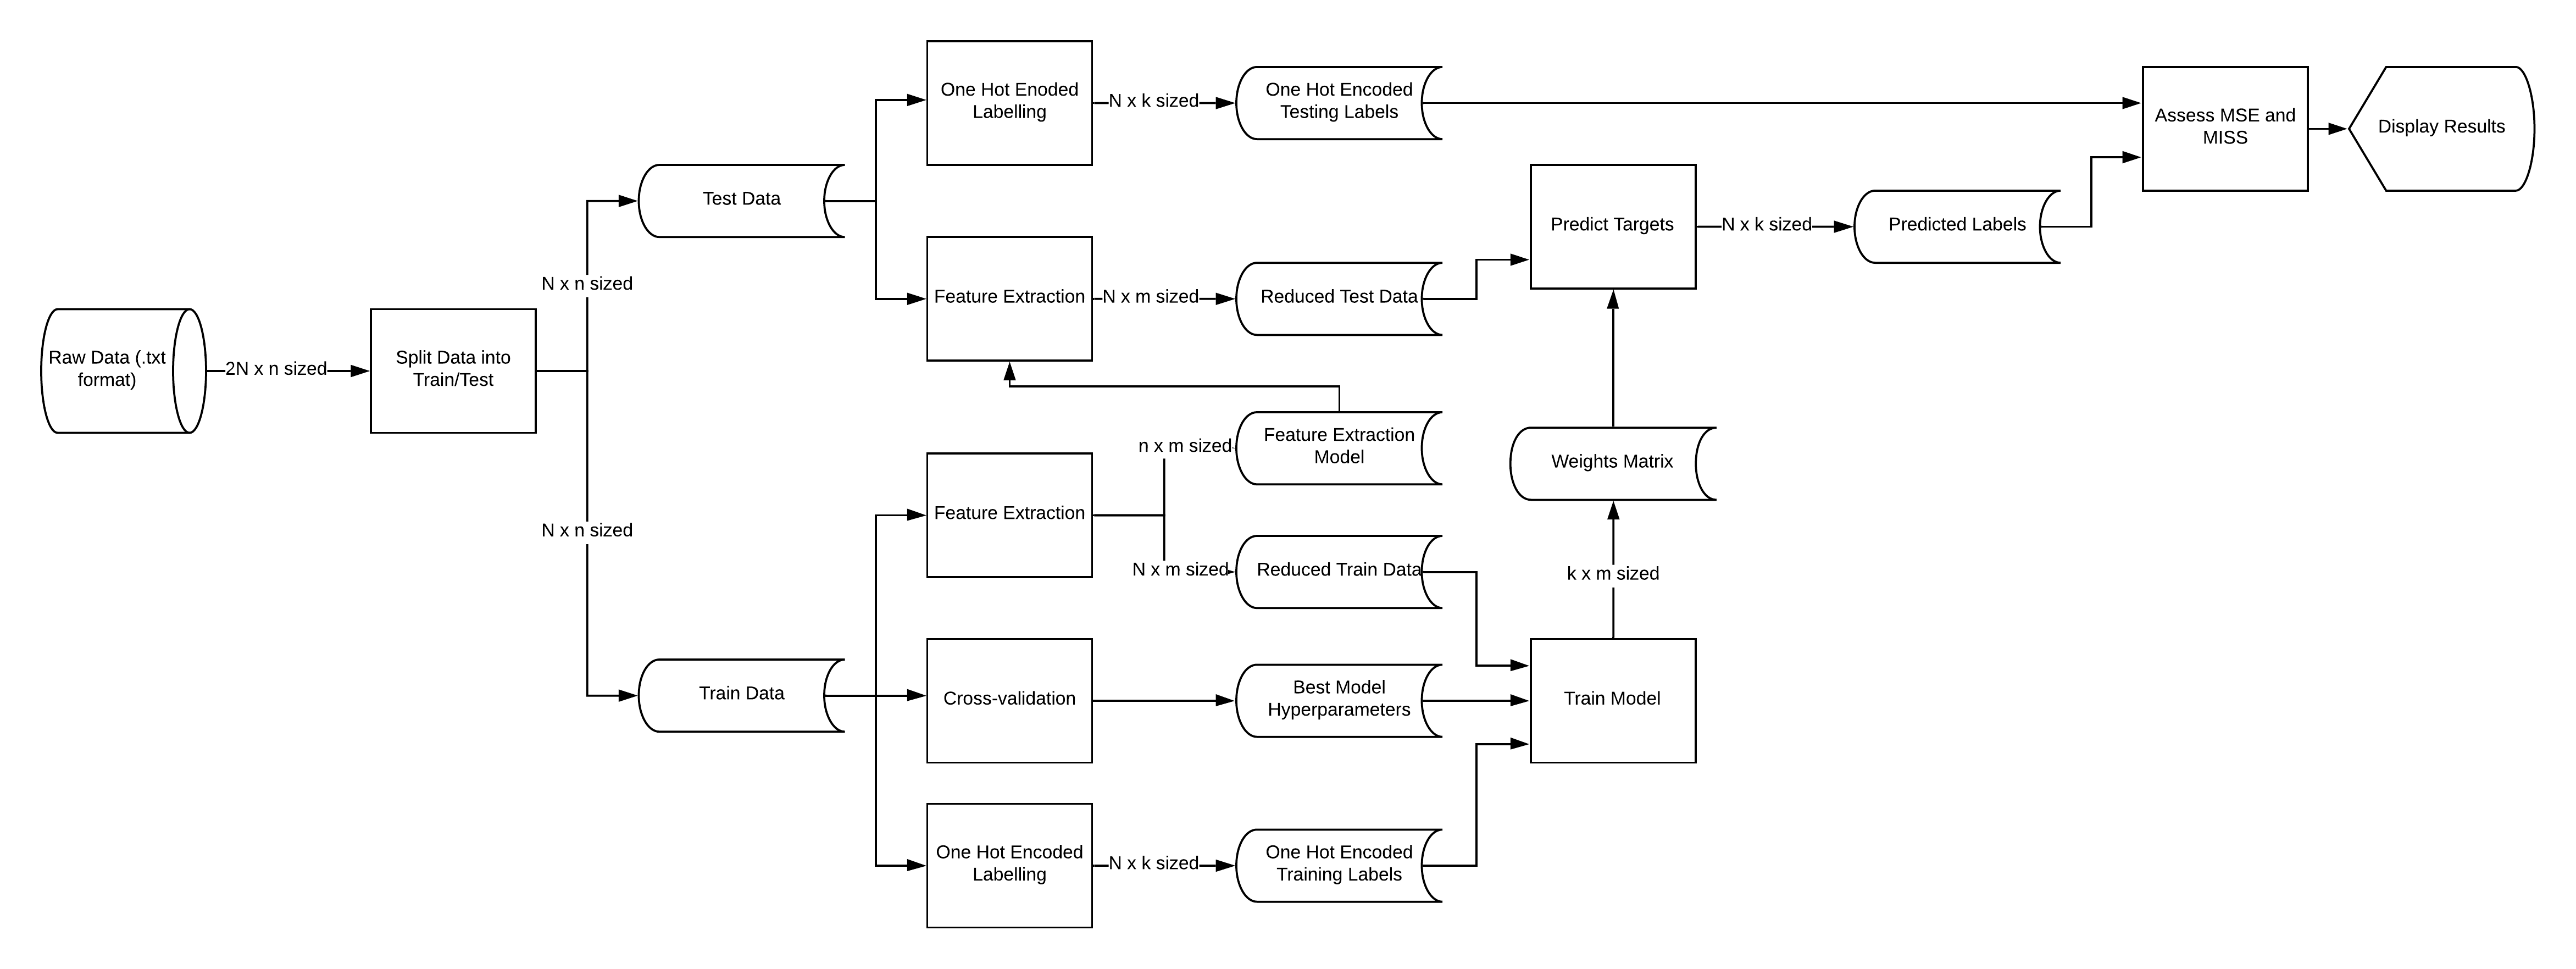
\includegraphics[scale=0.37]{images/pipeline.png}
    \caption{Full Data Processing Pipeline.}
    \label{fig:pipeline}
\end{figure}

\subsection{Implementation}

The data pipeline is implemented in the programming language Python. Some Python libraries are used as well to ease the process. They follow:

\begin{itemize}
    \item \textbf{\textit{numpy}}: for matrices and vector manipulation \parencite{ numpydot, numpyidentity, numpylinalgpinv};
    \item \textbf{\textit{matplotlib}}: for plots generation \parencite{matplotlibplot};
    \item \textbf{\textit{pandas}}: facilitate the visualization of the data in a tabular format \parencite{pandasdataframe}.

\end{itemize}

Apart from these Python libraries, some codes implemented in the first Machine Learning Miniproject are reused. For instance, the \textit{K-means} algorithm is completely reused as well as some auxiliary functions. For this, the previously-implemented code is arranged into the new file \textit{miniprojectone.py} and imported by the codes implemented in the Python project for this report.

The data processing pipeline is executed using a \textit{Jupyter Notebook} and then converted to a \textit{.py} file. A standalone \textit{.py} file is also created. This standalone file allows executing the pipeline, except for the grid search strategy, in order to validate the results to be mentioned yet in this report.

Being out of the scope of this project, we do not cover Unit Testing and Integration Testing\usepackage{} for the implemented code. That is to say, the code is maintained and tested throughout the outputs and the visualizations as expected. Hence,  for future updates or releases, the new implementation will demand that we reevaluate certain blocks of code by rerunning them.

\section{Analysis and Results}

The linear model is tested, through cross-validation, for different values of the hyperparameter $\alpha$ and the number of \textit{K-means} clusters. The results are present in the following subsections.

In addition, PCA is also applied during the feature extraction stage. Through cross-validation and a grid search strategy, the optimal values for the number of Principal Components and $\alpha$ are obtained.

\subsection{Feature Extraction Using \textit{K-Means}} \label{sec:k-means}

We begin our analysis with \textit{K-Means}.

\subsubsection{Cross-validation for Different Number of Clusters \textit{K}} \label{sec:cv_k_means}

Using \textit{K-fold} cross-validation, a range of the number of clusters are tested while seeking for the best value. In this testing scenario, the linear model parameter $\alpha$ is constantly set to 0. The results are then presented in Table \ref{table:diff_k}.

\begin{table}[h!]
\begin{center}
 \begin{tabular}{||c | c | c | c | c||} 
 \hline
 K & $MSE_{train}$ & $MISS_{train}$ (\%) & $MSE_{validate}$ & $MISS_{validate}$ (\%) \\ [0.5ex]
 \hline\hline
 2 & 0.767940 & 63.62 & 0.772451 & 64.1\\ 
 \hline
 5 & 0.612294 & 33.68 & 0.618742 & 35.3\\
 \hline
 10 & 0.402264 & 17.27 & 0.409435 & 17.3\\
 \hline
 20 & 0.227399 & 5.28 & 0.248641 & 5.9\\
 \hline
 50 & 0.159679 & 3.22 & 0.189419 & 3.5\\
 \hline
  100 & 0.119638 & 2.03 & 0.157589 & 3\\
 \hline
  200 & 0.084664 & 1.21 & 0.135771 & 3\\
 \hline
  400 & 0.049026 & 0.39 & 0.120286 & 2.4\\
 \hline
  800 & 0.006403 & 0 & 0.105101 & 1.8\\
 \hline
\end{tabular}
\caption{Linear model performance for different number of clusters.}
\label{table:diff_k}
\end{center}
\end{table}

The results presented in Table \ref{table:diff_k} are visualized as line plots in Figure \ref{fig:diff_k}.

\begin{figure}[h!]
    \centering
    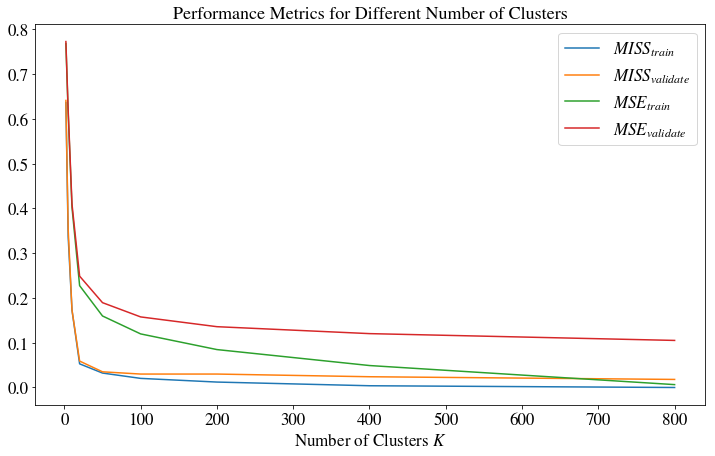
\includegraphics[scale=0.42]{images/cv_metrics.png}
    \caption{Linear model metrics varying the number of clusters.}
    \label{fig:diff_k}
\end{figure}

The results are somehow surprising. Increasing the number has caused the model to better perform in the training data and testing data, as all the four curves of Figure \ref{fig:diff_k} show. For the values higher than 200 clusters, such as 400 clusters and  800 clusters, the performance is even better in both scenarios, training and testing data. However, while this approach was possible in a practical way, that is, the $K$ parameter was set to 400 and 800 and the results collected, formally, strictly speaking, this strategy is incoherent, given that data dimensionality is being increased and not reduced.

In a sense, for these two particular cases, the feature extraction stage is creating new data (from 240 features to 400 or 800 features). One can argue that most of these features will be correlated between them. Most of the clusters will contain only one or two datapoints, that is, each cluster will determine a codebook similar, or very similar, to the data point itself. Consequently, data patterns similar (for instance group of the digits zero), will have correlated distances to the other redundant clusters. 

While adding more features into the training data theoretically may lead to overfitting given that model complexity is increased, our experimental case has shown the following: the more features the linear model has available in both training and testing scenarios, the better it performs.

\subsubsection{Cross-validation Varying the Ridge Factor $\alpha$}

The same procedure described in Section \ref{sec:cv_k_means} is utilized again, but this time by varying the ridge factor $\alpha$ and setting the number of clusters to 50. The results are presented in Table \ref{table:diff_alpha}.

\begin{table}[h!]
\begin{center}
 \begin{tabular}{||c | c | c | c | c||} 
 \hline
 $\alpha$ & $MSE_{train}$ & $MISS_{train}$ (\%) & $MSE_{validate}$ & $MISS_{validate}$ (\%) \\ [0.5ex]
 \hline\hline
 0 & 0.160896 & 3.33 & 0.188384 & 4.0\\ 
 \hline
 0.5 & 0.158641 & 3.37 & 0.187778 & 4.1\\
 \hline
 1.0 & 0.160887 & 3.24 & 0.188090 & 4.2\\
 \hline
 10.0 & 0.158483 & 3.29 & 0.185186 & 4.6\\
 \hline
 25.0 & 0.161007 & 3.33 & 0.190026 & 3.9\\
 \hline
  50.0 & 0.160162 & 3.21 & 0.190930 & 4.3\\
 \hline
  100.0 & 0.158552 & 3.29 & 0.187669 & 3.8\\
 \hline
  500.0 & 0.173398 & 3.53 & 0.200994 & 4.4\\
 \hline
  1000.0 & 0.185375 & 3.79 & 0.215305 & 4.6\\
 \hline
\end{tabular}
\caption{Linear model performance for different $\alpha$ values.}
\label{table:diff_alpha}
\end{center}
\end{table}

The results observed in Table \ref{table:diff_alpha} are visualized in the line plot illustrated by  Figure \ref{fig:diff_alpha}. The $\alpha$ parameter acts by limiting the linear model flexibility. This way, as Figure \ref{fig:diff_alpha} shows, increasing alpha will control the variance, but, for higher values, will also make the model biased. Inspecting Figure \ref{fig:diff_alpha} it is possible to notice that for $\alpha$ values higher than 200 the model start to present worse results both in the training and testing data.

For values lower than 250, there is no significant difference in the model performance in the training and testing data. This fact shows that the model does not overfit even if $\alpha$ is set to zero, once the results are satisfactory (according to our 96\% accuracy goal) and consistent in training and testing data.

\begin{figure}[h!]
    \centering
    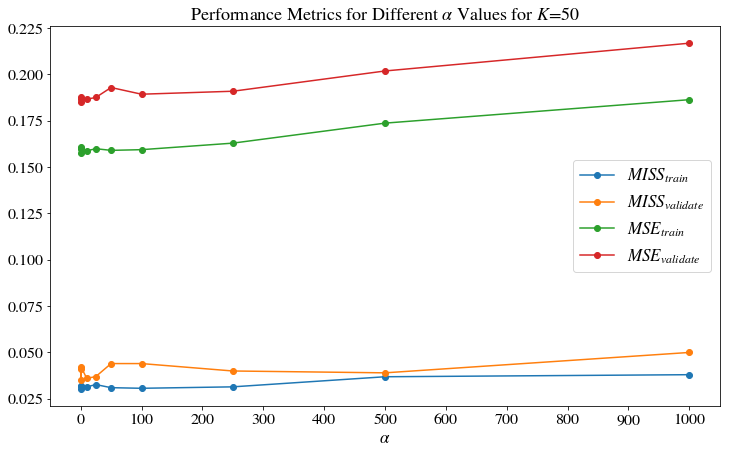
\includegraphics[scale=0.42]{images/cv_alpha.png}
    \caption{Linear model metrics varying the value set for $\alpha$.}
    \label{fig:diff_alpha}
\end{figure}

\subsection{Feature Extraction Using PCA}

The same procedure executed in Section \ref{sec:k-means} is repeated, but with PCA as the feature extraction function. This section covers the results obtained in this case.

\subsubsection{Cross-validation for Different Number of Principal Components}

Using \textit{K-fold} cross-validation, a range of the number of principal components are tested while seeking for the best value. In this testing scenario, the linear model parameter $\alpha$ is constantly set to 0. The results are then presented in Table \ref{table:diff_pc}.

\begin{table}[h!]
\begin{center}
 \begin{tabular}{||c | c | c | c | c||} 
 \hline
 PCs & $MSE_{train}$ & $MISS_{train}$ (\%) & $MSE_{validate}$ & $MISS_{validate}$ (\%) \\ [0.5ex]
 \hline\hline
 2 & 0.836181 & 63.49 & 0.839118 & 64.40\\ 
 \hline
 10 & 0.521497 & 15.90 & 0.535045 & 17.10\\
 \hline
 20 & 0.382183 & 7.94 & 0.401805 & 9.60\\
 \hline
 40 & 0.314818 & 5.56 & 0.346266 & 7.40\\
 \hline
 50 & 0.304419 & 5.52 & 0.344324 & 7.80\\
 \hline
  60 & 0.295735 & 4.79 & 0.340446 & 7.20\\
 \hline
  80 & 0.279795 & 4.24 & 0.340578 & 7.30\\
 \hline
  100 & 0.269948 & 4.14 & 0.339192 & 7.10\\
 \hline
  125 & 0.258100 & 3.56 & 0.348397 & 7.50\\
 \hline
  150 & 0.247287 & 3.31 & 0.356946 & 8.10\\
 \hline
  175 & 0.236994 & 3.04 & 0.371753 & 9.40\\
 \hline
  200 & 0.228009 & 2.50 & 0.378591 & 8.50\\
 \hline
  239 & 0.214497 & 1.87 & 0.404585 & 8.70\\
 \hline
\end{tabular}
\caption{Linear model performance for different number of principal components.}
\label{table:diff_pc}
\end{center}
\end{table}

The results presented in Table \ref{table:diff_pc} are visualized as line plots in Figure \ref{fig:diff_principal}.

\begin{figure}[h!]
    \centering
    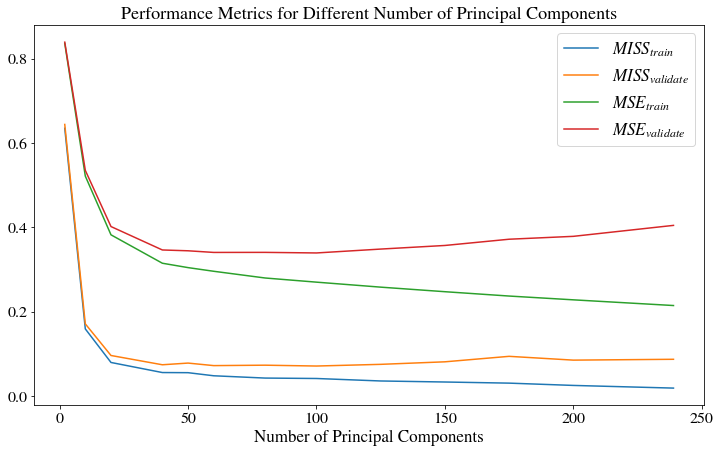
\includegraphics[scale=0.42]{images/cv_pcs.png}
    \caption{Linear model metrics varying the number of principal components.}
    \label{fig:diff_principal}
\end{figure}

Through inspection in the curves showen in Figure \ref{fig:diff_principal}, it is possible to detect that increasing the number of principal components causes that model to overfit, given that $MSE_{train}$ keeps steadily decreasing.  Meanwhile, $MSE_{test}$ starts to increase after around 50 principal components.

\subsubsection{Cross-validation Varying the Ridge Factor $\alpha$}

As Figure \ref{fig:diff_principal} has shown, after some point, the model overfits for higher numbers of principal components. Therefore, we try here to control the model overfitting by experimenting with different values of $\alpha$ and setting the number of principal components to the constant value of 80. The results obtained are presented in Table \ref{table:diff_pc_alpha}.

\begin{table}[h!]
\begin{center}
 \begin{tabular}{||c | c | c | c | c||} 
 \hline
 $\alpha$ & $MSE_{train}$ & $MISS_{train}$ (\%) & $MSE_{validate}$ & $MISS_{validate}$ (\%) \\ [0.5ex]
 \hline\hline
 0 & 0.279800 & 4.133333 & 0.339638 & 7.2\\ 
 \hline
 0.5 & 0.280011 & 4.166667 & 0.337632 & 7.3\\
 \hline
 1.0 & 0.279984 & 4.222222 & 0.339234 & 7.5\\
 \hline
 10.0 & 0.280020 & 4.177778 & 0.338284 & 7.2\\
 \hline
 25.0 & 0.279950 & 4.144444 & 0.339941 & 7.1\\
 \hline
  50.0 & 0.280084 & 4.133333 & 0.335431 & 7.0\\
 \hline
  100.0 & 0.279933 & 4.133333 & 0.339405 & 7.4\\
 \hline
  250.0 & 0.280488 & 4.333333 & 0.335124 & 7.5\\
 \hline
  500.0 & 0.281786 & 4.311111 & 0.334209 & 7.2\\
 \hline
  1000.0 & 0.285533 & 4.500000 & 0.332705 & 7.7\\
 \hline
\end{tabular}
\caption{Linear model performance for different $\alpha$ values with 80 principal components.}
\label{table:diff_pc_alpha}
\end{center}
\end{table}

The results presented in Table \ref{table:diff_pc_alpha} are visualized as line plots in Figure \ref{fig:diff_pc_principal}.

\begin{figure}[h!]
    \centering
    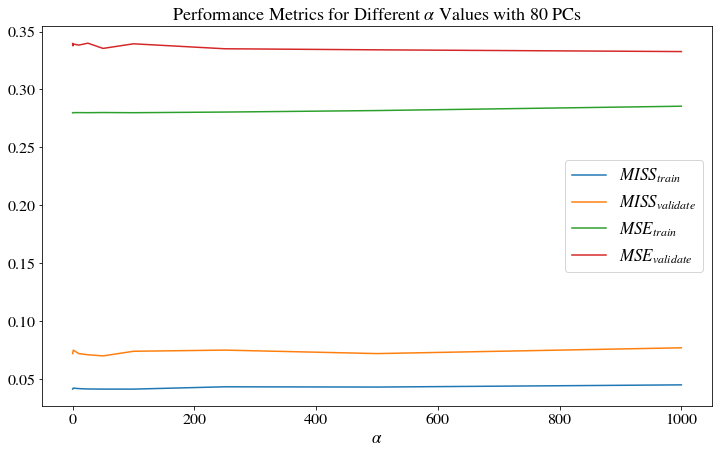
\includegraphics[scale=0.42]{images/cv_pcs_alpha.png}
    \caption{Linear model metrics varying $\alpha$ with 80 principal components.}
    \label{fig:diff_pc_principal}
\end{figure}

Visually speaking, we do not appreciate any clear effect of the $\alpha$ parameter in the model performance. The results are practically constant over the $\alpha$ values range. We check this claim by the almost constant lines in Figure \ref{fig:diff_pc_principal}.

\subsection{\textit{K-means} and PCA Processing Times Comparison}
During the cross-validation stage, the time spent for a full cross-validation test is stored for both feature extraction scenarios: \textit{K-means} and PCA. The results obtained are presented in Table \ref{table:times}. To make the comparison fair, we set both the number of clusters and principal components to 100.

\begin{table}[h!]
\begin{center}
 \begin{tabular}{||c | c||} 
 \hline
 \textit{K-means} Processing Time (\textit{s}) & PCA Processing Time (\textit{s}) \\ [0.5ex]
 \hline\hline
  324.13 & 0.48\\ 
 \hline
\end{tabular}
\caption{Comparison of \textit{K-means} and PCA Processing Time as Feature Extractor in a cross-validation.}
\label{table:times}
\end{center}
\end{table}

While \textit{K-means} outperforms PCA, considering only the metrics scores, PCA is almost 1000 times faster. This fact can be relevant in applications where the training processing time is critical. 

\subsection{Model Validation on the Test Data}

Considering the best results obtained during the cross-validation (results presented in Tables \ref{table:diff_k} and \ref{table:diff_alpha}, a reasonable model is selected. By reasonable, we mean a model that presents good results (above 96\% of accuracy) and still makes statistical sense. Also, the number of clusters is chosen by taking into account the \textit{K-means} processing time, as a higher number of cluster means slower processing time. In this sense, Table \ref{table:best_linear} describes the parameters for this model.

\begin{table}[h!]
\begin{center}
 \begin{tabular}{||c | c||} 
 \hline
 $\alpha$ & \textit{K} \\ [0.5ex]
 \hline\hline
 0.0 & 100\\ 
 \hline
\end{tabular}
\caption{Chosen linear model parameters.}
\label{table:best_linear}
\end{center}
\end{table}

This model is then evaluated on the Test Data. It is worth mentioning that the Test Data is not processed during the training and cross-validation stages, as illustrated by the pipeline in Figure \ref{fig:pipeline}. In other words, it can be considered as a dataset completely new.

The results obtained for the Test Data are arranged in Table \ref{table:best_linear_metrics}. For the sake of comparison, the results obtained with the same configuration described in Table \ref{table:best_linear} during cross-validation are presented in the bar plot presented in Figure \ref{fig:metrics_comparison}. However, we should make clear that these results are not deterministic given that random seed configuration was implemented in this project.

\begin{table}[h!]
\begin{center}
 \begin{tabular}{||c | c||} 
 \hline
 $MSE_{test}$ & $MISS_{test} (\%)$ \\ [0.5ex]
 \hline\hline
  0.1509 & 3.0\\ 
 \hline
\end{tabular}
\caption{Chosen linear model performance on the Test Data.}
\label{table:best_linear_metrics}
\end{center}
\end{table}

\begin{figure}[h!]
    \centering
    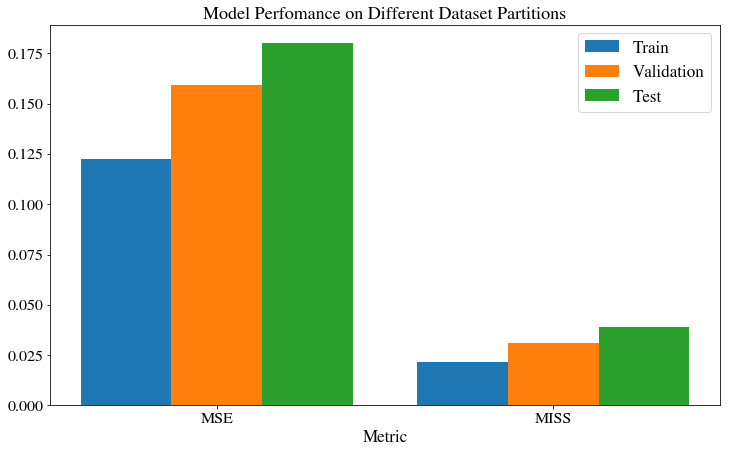
\includegraphics[scale=0.42]{images/metrics_comparison.png}
    \caption{Model metrics in training data, validating data and testing data.}
    \label{fig:metrics_comparison}
\end{figure}

Figure \ref{fig:metrics_comparison} shows that the cross-validation is very efficient is estimating the MISS and MSE metrics in a new dataset. The results obtained with the Test Data are very similar to the results obtained in cross-validation.

Soon, as expected, cross-validation is a useful statistical method that allows one to estimate the model performance when only a limited amount of training data is available or the test data is unavailable. This situation is common in real-world applications where the procedure to produce new data are either costly or even unfeasible. 

\section{Conclusion}

In the project presented in this report, a full data processing pipeline is implemented. Beginning with the loading of the data, feature extraction for dimensionality reduction and finally, a linear model is applied. Different methods are tested in the feature extraction stage and hyperparameters involved are optimized by a grid search strategy. The model with the best performance is then applied to an entirely new dataset.

The model presented better performance using \textit{K-means} reduction in the feature extraction stage in comparison to PCA. The model obtained excellent results even for a higher number of features, 800 features for instance. However, we decided to use a more feasible number of features, such as 100 features, in the best model. 800 features do not make sense, formally speaking, as this means that feature extraction is increasing the number of features. So one may conjecture that for this high number of features, most of them will be highly correlated.

While \textit{K-means} performed satisfactorily regarding the metrics scores, the same cannot be extended to its processing time performance. In this sense, \textit{K-means} reduction is almost 1000 times slower than PCA reduction. Thereby, for cases where processing time has higher or equal weight than the metrics scores, PCA presents itself as a powerful solution, since it is significantly faster without highly compromising the metrics performance.

Finally, the cross-validation presented itself as an important technique for estimating the model performance in the test data. This way, during the training stage, it is possible to consistently evaluate the model performance on unseen data using only the training data available. This characteristic can be useful in applications where no testing data is available.

% REFERENCES
\clearpage
\newpage
\printbibliography

\end{document}

